% Chapter Template

\chapter{Theory} % Main chapter title
This chapter focuses on explaining the general theory behind the model and the methods used in this work.
Details regarding the exact problem definition, model adjustments, programs used and so on are given in
\hyperref[chap:methods]{Chapter \ref*{chap:methods}}.


\label{chap:theory} % Change X to a consecutive number; for referencing this chapter elsewhere, use \ref{ChapterX}

%----------------------------------------------------------------------------------------
%	SECTION 1
%----------------------------------------------------------------------------------------

\section{Compartmental modeling techniques}
Compartmental modeling revere to a modeling technique often used to systematically describe real world phenomena
like disease spreading\cite{compartementMod}. In these models the population is divided into different groups. 
Members of one group can move to another group. This movement is based on equations that are used to model the real
world behavior of each group. The following two sections introduce both the ``SIR'' and the ``SEIRD'' model. The
latter model was the focus on this work.

%-----------------------------------
%	SUBSECTION 1
%-----------------------------------
\subsection{Ordinary differential equations}

%-----------------------------------
%	SUBSECTION 2
%-----------------------------------
\subsection{Partial differential equations}


%-----------------------------------
%	SUBSECTION 3
%-----------------------------------
\subsection{The SIR model}
\label{sec:SIR}
In 1927 \cite{kermack1991contributions} first introduced their method to mathematically describe  
the course  of an infectious disease. The model divides a population into three distinct groups.

\begin{enumerate}[label=$\bullet$]
	\item \B{Susceptibles (S)}: Individuals that are naive to the infection and hence not immune. If in contact with
		the virus these individuals can migrate to the\linebreak ``Infected'' group
	\item \B{Infected (I)}: Individuals that are infected with the disease. Infected individuals contribute to the 
		infection of members of the susceptible group. At some point during their infection, these members
		transition to the ``Removed'' group.
	\item \B{Removed (R)}: Individuals that  have either overcome their infection and are now immune to the disease
		or have succumb to the disease and are diseased. They do not spread the virus and cannot be infected again.
\end{enumerate}

\par
The population changes of all three groups are described by mathematical equations\cite{mathSIR}. Notable variables
are the number of susceptible members (S), number of infected members (I), number of recovered members (R), $\alpha$
which is a positive constant that describes the transmission rate of the disease and $\beta$, which is a positive
constant between 0 and 1 that describes the transition rate (either recovery or death) between \B{I} and \B{R}.
$\beta$ can be rewritten as $\frac{1}{b}$, where $b$ is the average duration an infected individual remains contagious,
before it either recovers or dies. The model is illustrated in \hyperref[fig:SIR]{Figure \ref*{fig:SIR}}, the equations
are expressed as follows:

\begin{figure}
	\begin{center}
		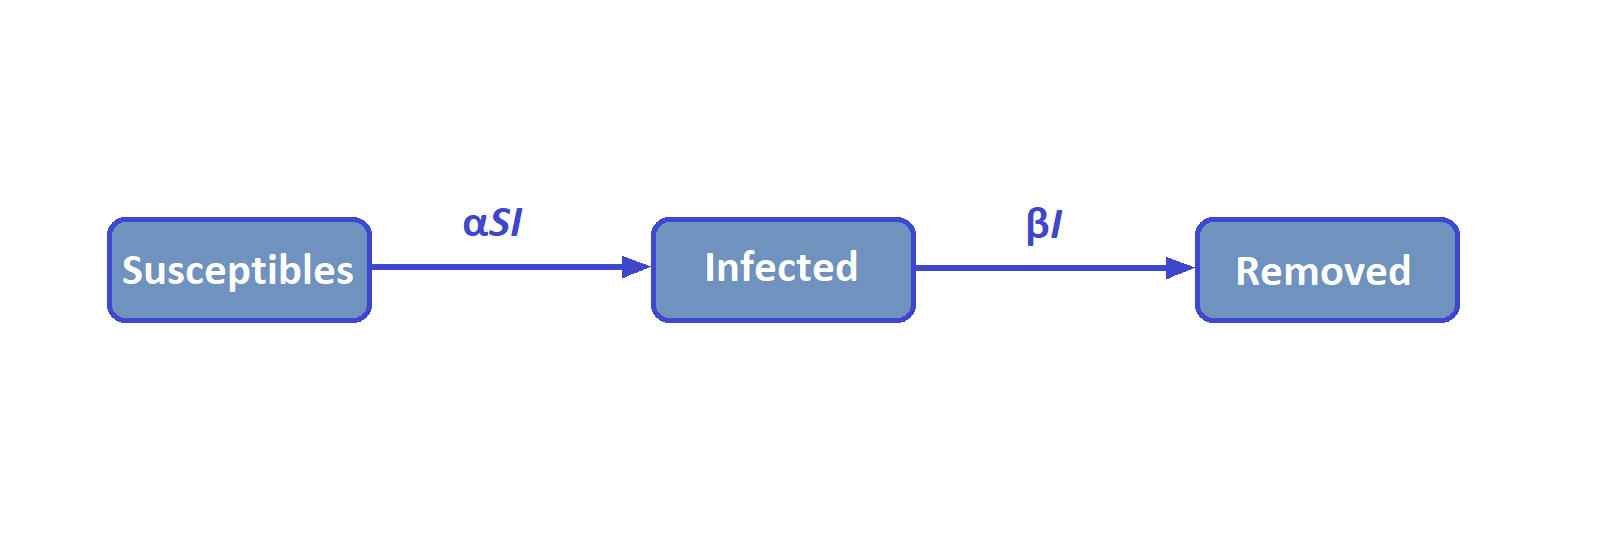
\includegraphics[width=0.75\textwidth]{./figures/SIR.png}
		\caption{Illustration of the population flow in the SIR model. S represents the ``Susceptible'', I
			the ``Infected'' and R the ``Removed'' population. The variable $\beta$ can also redefined
			as $\frac{1}{b}$, where $D$ is the average duration of contagiousness}
		\label{fig:SIR}
	\end{center}
\end{figure}


\begin{align}
	\label{eq:SIR1}
	\frac{dS}{dt} &= -\alpha S I \\
	\frac{dI}{dt} &= \alpha S I - \beta I \\
	\frac{dR}{dt} &= \beta I
\end{align}

\par
The model also assumes the total number of individuals in the system $N$ remains constant and that the sum of all transitions
between all three groups during every time step remains zero. This is expressed in the equations below.
$S(t)$, $I(t)$ and $R(t)$ express the number of individuals in each of the groups, at time $t$, respectively.

\begin{align}
	\label{eq:SIR2}
	I(t) + S(t) + R(t) &= N \\
	\frac{dS}{dt} + \frac{dI}{dt} + \frac{dR}{dt} = 0
\end{align}

\par
Since the model assumes, that the total population remains stable, phenomena like immigration or child birth are not accounted
for. This does not correctly represent the real world. However it is often assumed, that population fluctuations
due to these occurrences are minor enough compared to the entirety of a regions population, that they do not alter the results of the
simulation in a major way\cite{??}.\newline

\par
In order to correctly model the dynamics of an epidemic, the variables of these differential
equations (like $\alpha$ and $\beta$ in this case) must be determined correctly. This process is referred to as solving the equations.
Different techniques exist to do so. Two of these techniques are the \hyperref[sec:Gauss]{Gauss-Newton algorithm}\cite{Gauss??} and
\hyperref[sec:PSO]{Particle Swarm Optimization (PSO)}\cite{PSO??}. Both of these techniques will are explained in a later section.


%-----------------------------------
%	SUBSECTION 4
%-----------------------------------

\subsection{The SEIRD model}
\label{sec:SEIRD}
The SEIRD model is a variant of the simpler SIR model\cite{knodel20173d}
\textcolor{red}{(double check citation)}. % note
It introduces two new groups and describes the status for the infected population much more precise. The groups of the SEIRD
model are as follows:

\begin{enumerate}[label=$\bullet$]
	\item \B{Susceptibles (S)}: Individuals that are naive to the infection and hence not immune (identical to SIR).
	\item \B{Exposed (E)}: Individuals that are infected, but show no or very little symptoms. These individuals
		do not quarantine (yet) and are therefor contributing to the spread of the virus.
	\item \B{Infected (I)}: Individuals that have developed such a sever illness, that they need to be hospitalized.
	\item \B{Recovered (R)}: Individuals that  have overcome the infection and are now immune to the disease.
	\item \B{Diseased (D)}: Individuals that have succumb to the infection.
\end{enumerate}

\par
As described in the previous section, transition between the Individuals of different groups is a core
part of the model. The transition between the \B{S} and \B{E} population in SEIRD is equivalent to the transition
between \B{S} and \B{I} in SIR. However, the population outflow from the \B{E} group is split and can either move
to the \B{I} or to the \B{R} group. This allows the modeling of infections that result in quick recovery or an infection
with complications (defined by the hospitalization of the patient). The ratio between the two scenarios is governed by the variable
$\kappa$. In addition, the variable $q$ was introduced and now represents the average duration until recovery/hospitalization of an
infected individual. Similarly, the outflow of \B{I} is split between the populations of \B{R} and \B{D}. The ratio is governed
by the variable $\tau$. The equations for \B{R} and \B{D} were also adjusted to represent these changes. Lastly $D$ was redefined
as $p$, which now represents the average of a hospitalized individual to either recover or succumb to the infection.
\hyperref[fig:SEIRD]{Figure \ref*{fig:SEIRD}} illustrates all these changes. The modified equations are as follows:

\begin{align}
	%\label{eq:SEIRD1}
	\frac{dS}{dt} &= -\alpha S E \label{eq:SEIRD1_S} \\
	\frac{dE}{dt} &= \alpha S E -\frac{1}{q} E \label{eq:SEIRD1_E} \\
	\frac{dI}{dt} &= \frac{\kappa}{q} E - \frac{1}{p} I \label{eq:SEIRD1_I} \\
	\frac{dR}{dt} &= \frac{1-\kappa}{q} E + \frac{1-\tau}{p} I \label{eq:SEIRD1_R} \\
	\frac{dD}{dt} &= \frac{\tau}{p} I \label{eq:SEIRD1_D} 
\end{align}


\begin{figure}
	\begin{center}
		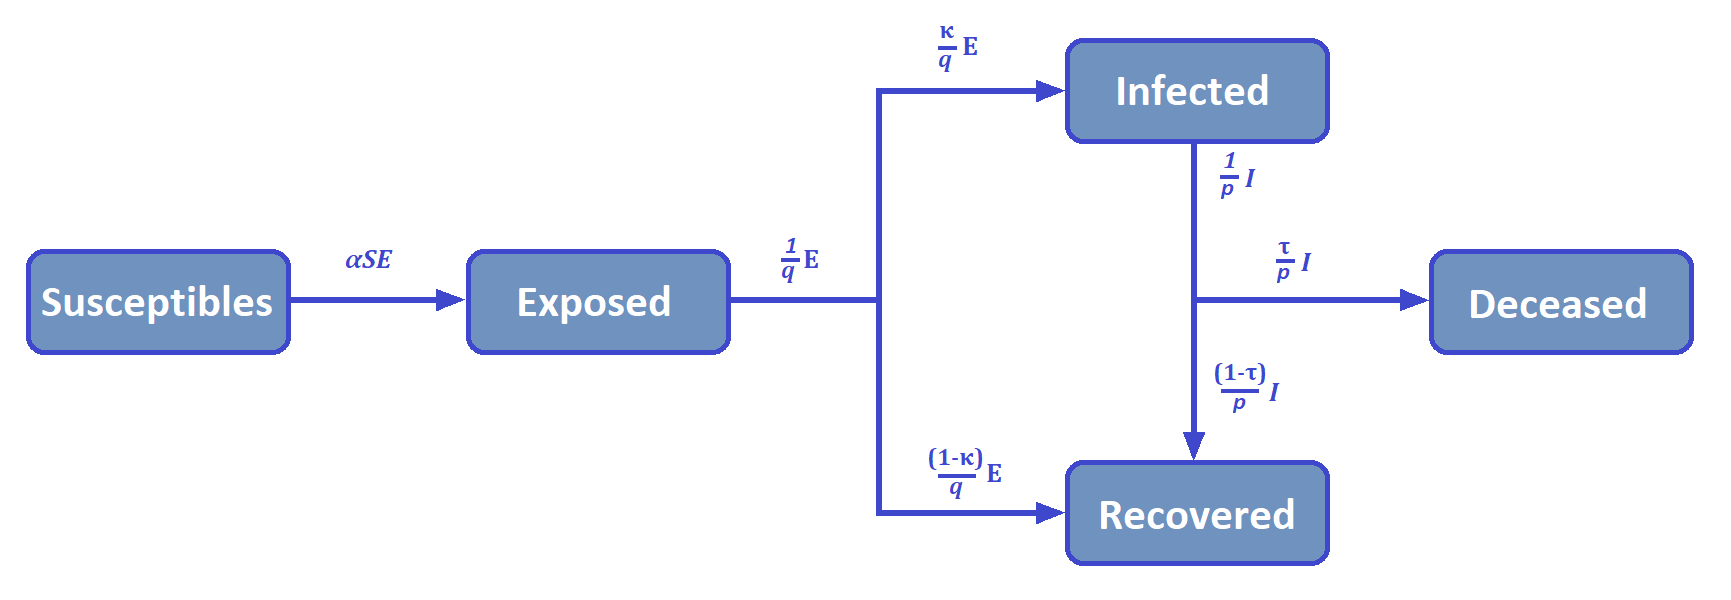
\includegraphics[width=0.75\textwidth]{./figures/SEIRD.png}
		\caption{Illustration of the population flow in the SEIRD model. S represents the ``Susceptible'', E the ``Exposed'',
			I the ``Infected'', R the ``Recovered'' and D the ``Diseased'' population. $\beta$ can also be expressed as
			$\frac{1}{\phi}$, where $\phi$ is the average time to recovery/hospitalization.}
		\label{fig:SEIRD}
	\end{center}
\end{figure}


\par
Like SIR, the SEIRD model assumes that the total number of individuals $N$ in the population remains constant during every step
of the modeling process. This leads to the equations expressed below. Again, $S(t)$, $E(t)$, $I(t)$, $R(t)$ and $D(t)$ are
expressing the number of individuals for each group at time $t$, respectively. $N$ remains the total number of individuals in the model.

\begin{align}
	\label{eq:SEIRD2}
	S(t) + E(t) + I(t) + R(t) + D(t) &= N \\
	\frac{dS}{dt} + \frac{dE}{dt}  + \frac{dI}{dt} + \frac{dR}{dt} + \frac{dD}{dt} = 0
\end{align}

\par
A model like this expresses the dynamics of an epidemic in much more detail. A weakness of the SIR model is that it does distinct between important
groups such as sick, but not infected and hospitalized individuals. The SEIRD model is capable of doing so and also allows for predicting
figures like the number of hospitalized individuals at time $t$.\newline

\par
This work focused mostly on the modeling capability of SIR in the transition stage between susceptibles and exposed. To better fulfill this
task, the model was redefined to accommodate for a lack of clear source data and to further refine the modeling of real wold phenomena. The changes
are described in detail in \hyperref[sec:SEIRDredef]{chapter~\ref*{chap:methods}, section~\ref*{sec:SEIRDredef}}.



%----------------------------------------------------------------------------------------
%	SECTION 2
%----------------------------------------------------------------------------------------

\section{Variable optimization algorithms}
In order for the presented models to work properly, it is important to determine the correct value for each unknown variable. There are many
methods to determine these variables. In the context of differential equations this process is often referred to as ``solving'' the equations.
Algorithms and methods that try to achieve this are generally referred to as ``solvers''.
The following sections will explain two methods used in this work. The Gauss-Newton algorithm and the Particle Swarm Optimization algorithm (PSO).

%-----------------------------------
%	SUBSECTION 1
%-----------------------------------

\subsection{Gauss-Newton algorithm}
\textcolor{red}{add citations, explain least squared better/at all}
\textcolor{red}{describe efficiency and why it is cool}
\label{sec:Gauss}
The Gauss-Newton algorithm is an iterative method, that is used to solve non-linear least square problems. Given a set of $m$ functions, $n$
variables that are used to calculate the function results  and a number of target values, the algorithm is used to optimize the variables in
such a way, that difference between function results and target values are minimized.\newline

The relevant parameters in this algorithm are the vector function $F(\theta)$, the Jacobian matrix $J$, the target values $X$ and the
estimated parameters $\theta^{i}$, the estimation change $\Delta^{i}$ and the error value $\epsilon^{i}$ of iterations $i$. Given $m$
functions and $n$ variables, with the condition that $m \geq n$, the definitions for $F(\theta)$, $\theta^{i}$, $\Delta^{i}$ and
$\epsilon^{i}$ are as follows.

\begin{align}
	F(\theta) =& (f_0(\theta), f_1(\theta),...,f_m(\theta))^T \\
	\theta^{i} =& (\theta^{i}_0, \theta^{i}_1, \theta^{i}_2,...,\theta^{i}_n)^T \\
	\Delta^{i} =& (\theta^{i}_0 - \theta^{i-1}_0, \theta^{i}_1 - \theta^{i-1}_1, ..., \theta^{i}_m - \theta^{i-1}_m)^T \\ %questionable?
	\epsilon^{i} =& F(\theta^{i}) - X
\end{align}

$F(\theta)$ is calculated iterative thought the algorithm and can be expressed in the form of a Taylor Series (eq. \ref*{eq:taylor1}) and
then rewritten as the Jacobian matrix $J$.

%note maybe add colors later
\begin{align}
	F(\theta^{i+1}) = F(\theta^{i} + \Delta^{i}) =&
		\begin{pmatrix} f_0(\theta^{i}) &+& \frac{\delta f_0(\theta)}{\delta \theta_0} \Delta^{i}_0 &+& ... &+&  \frac{\delta f_0(\theta)}{\delta \theta_n} \Delta^{i}_n  \\
				. && && && . \\
				. && && && . \\
				f_m(\theta^{i}) &+& \frac{\delta f_0(\theta)}{\delta \theta_0} \Delta^{i}_0 &+& ... &+&  \frac{\delta f_m(\theta)}{\delta \theta_n} \Delta^{i}_n 
		\end{pmatrix} \label{eq:taylor1} \\
	=& \begin{pmatrix} f_0(\theta^{i}) \\ . \\ . \\ f_m(\theta^{i})  \end{pmatrix} +
		\begin{pmatrix} \frac{\delta f_0(\theta)}{\delta \theta_0} & . & . & \frac{\delta f_0(\theta)}{\delta \theta_n}  \\
					   . &&& . \\
					   . &&& . \\
					   \frac{\delta f_m(\theta)}{\delta \theta_0} & . & . & \frac{\delta f_m(\theta)}{\delta \theta_n}
		\end{pmatrix} \begin{pmatrix} \Delta^{i}_0 \\ . \\ . \\ \Delta^{i}_n \end{pmatrix}  \label{eq:taylor2} \\
	=& F(\theta^{i}) + J \Delta^{i} \label{eq:taylor3}
\end{align}

This means the Jacobian Matrix $J$ is defined as such

\begin{align}
	J_{pq} = \frac{\delta f_p(\theta)}{\delta \theta_q} \quad \text{where } \quad p \in \{0,1,..,m\},\text{ } q \in \{0,1,...,n\}
\end{align}

To minimize the error $\epsilon$ in each following iteration, a connection is established between the current error and the
error of the following iteration, such that the non-linear least squared method can be used. This process is shown below.

\begin{align}
	& \epsilon^{i+1} = F(\theta^{i} + \Delta^{i}) - X \quad \text{since} \quad F(\theta^{i} + \Delta^{i}) = F(\theta^{i}) + J \Delta^{i} \\
	\Leftrightarrow & \epsilon^{i+1} = F(\theta^{i}) + J \Delta^{i}) - X \quad \text{since} \quad \epsilon^{i} = F(\theta^{i}) - X \\
	\Leftrightarrow & \epsilon^{i+1} = \epsilon^{i} + J \Delta^{i} \label{eq:taylor4}
\end{align}

Since the goal is to minimize the epsilon of the following iteration, equation \ref*{eq:taylor4} can be set equal to zero and reorganized to
take the form of a linear equation $Ax = b$. Since $\Delta$ steps usually are sufficiently small, it is assumed that the function is locally
linear. The non-linear least square method is then used to calculate $\Delta$ of the following equation.

\begin{align}
	&\text{min} \| \epsilon^{i} + J \Delta^{i} \| \\
	\Rightarrow & \epsilon^{i} + J \Delta^{i} = 0 \\
	\Leftrightarrow & J \Delta^{i} = -\epsilon^{i} \qquad \text{since $Ax = b$, least squared: } x = (A^T A)^{-1} A^T b \\
	\Leftrightarrow & \Delta^{i} = - (J^T J)^{-1} F^T \epsilon^{i} \label{eq:taylor5}
\end{align}

Therefor equation \ref*{eq:taylor5} can be used to calculate a suitible $\Delta$ in order to decrease the error in each iteration. \newline

The core steps of the Gauss-Newton method are listed below as pseudo-code.

%\begin{enumerate}
%	\item Start with an initial estimate $\theta^{(0)}$ for the optimal variables
%	\item Calculate the error $\epsilon$ between the target data and the function results with the estimated values. If $\epsilon$
%		is not zero or fulfills a breaking condition, continue. Otherwise return the current estimate 
%	\item Calculate the Jacobian-Matrix $J$ using the functions and the current estimate
%	\item Use $J$ and $\epsilon$ to calculate the difference $\Delta$ by which the estimate of the current iteration is
%		modified. Update the current estimate and continue from step 2
%\end{enumerate}


\begin{algorithm}
	\caption{Gauss-Newton algorithm pseudocode}
	Initialize estimate $\theta^{(0)}$ for the optimal variables;
	Calculate initial error $\epsilon^0$;
	Set i=0;
	\While {$\epsilon^i$ != 0 \Or (breaking conditions not fulfilled)}
		\State Calculate the Jacobian-Matrix $J$ using $\theta^i$;
		\State Use $J$ and $\epsilon^i$ to calculate estimate adjustment $\Delta^i$;
		\State Set i=i+1;
		\State Calculate $\epsilon^i$
	\EndWhile
	Return $\theta^i$;
\end{algorithm}


%-----------------------------------
%	SUBSECTION 2
%-----------------------------------

\subsection{Particle Swarm Optimization}
\label{sec:PSO}
Like the Gauss-Newton algorithm, $Particle Swarm Optimization$ (PSO) is a method used to iteratively optimize a problem. The general
concept of PSO is to generate a number of candidate solutions (particles) per iteration, quantify the quality of each solution, take the best
candidate of the sum of all particles (swarm) as the current best solution and try to improve this solution in following iterations.
Improvements are made by (randomly) altering the candidate solutions in hopes of finding a new solution, that improves on the previous best.
If suitable breaking conditions are met or the maximum number of iterations has passed, the algorithm stops and returns the current best solution.
In order to find the best solution in the defined search space as quickly and efficiently as possible, additional conditions are applied
to each particle. Particles are grouped together and a current best group solution is recorded, in addition to the current global optimal solution.
Modifications of the solution of each particle per iteration are still random, but in some way biased towards both the group and global optimum.
This is meant to direct a greater number of particles to the area of the most optimal solutions, that are currently known.
However, these solution may not be the global optimum for the defined search space and there is no guarantee, that improvements will be made in any
given iteration. As a trade off, the problem function does not need to be differentiable like it is the case for the Gauss-Newton algorithm. \newline

There are many different types of PSO algorithms. The following is a general setup:\newline
A problem space is defined, as well as a cost function $L$, which takes a number of $n$ input values in the from of a vector $\theta$ and projects them
to a real number $\epsilon$. The goal is to minimize this function. Each particle $p_i$ is defined by a number of variables. These variables are its candidate
solution (also called position) $position_i$, the positional change of the particle $velocity_i$, the current best group solution $best_group_i$, the
current best global solution $best_swarm_i$ as well as its group index $group_i$.

\begin{align}
	
\end{align}



